\chapter{Symmetry and SAT}\label{chap:symmetryinsat}


Despite SAT solving is an NP complete algorithm it works well on many real industrial problems. This is 
principally due to capacity to cut off search space with learning clause. Another ways to cut off 
search space is the exploitation of symmetry. Some instances exhibit symmetries and not taking them into account 
forces solvers to needlessly explore isomorphic search space.  \hakan{symmetrie leaves object invariant}




\section{Groups basics}

As symmetries is a belongs to a branch of mathematics called theory group.
This section give us an overview of group theory.


\subsection{Groups}

A \emph{group} is a structure $\langle G, * \rangle$, where $G$ is a non empty set and $*$ a binary
operation such the following axioms are satisfied:
\begin{itemize}[noitemsep,nolistsep]
	\item \emph{associativity}: $\forall a, b, c \in G, (a * b) * c = a * (b * c)$
	\item \emph{closure}: $\forall a, b \in G, a * b \in G$.
	\item \emph{identity}: $\forall a \in G, \exists e$ such that $ a * e = e * a = a$
	\item \emph{inverse}:  $\forall a \in G, \exists b \in G$, commonly denoted $a^{-1}$ such that
	$a * a^{-1} = a^{-1} * a = e$
\end{itemize}

Note that \emph{commutativity} is not required i.e $\ a * b = b * a$, for $a, b \in G$.
The group is \emph{abelian} if it satisfies the commutativity rule.
Moreover, the last definition leads to important properties which are: i) uniqueness of the identity element. 
To prove this property, assume $\langle G, * \rangle$ a group with two identity elements $e$ and $f$ 
then $ e = e * f = f$.
ii) uniqueness of the inverse element. To prove this property, suppose that an element $x_1$ has two inverses,
denoted $b$ and $c$ in group $\langle G, * \rangle$, then\\
$\begin{array}{lcll}					
b & = & b * e & \\
& = & b * (a * c) & c \text{ is an inverse of } a, \text{so } e = a * c\\
& = & (b * a) * c &   \text{\emph{associativity} rule}\\
& = & e * c       & b \text{ is an inverse of } a, \text{so } e = a * b\\
& = & c           &   \text{\emph{identity} rule}
\end{array}$

The structure $\langle G, * \rangle$ is denoted as G when clear from context that G is a group
with a binary operation. In this thesis, we interested only with the \emph{finite} groups i.e
with a finite number of elements.

Given a group $G$, a \emph{subgroup} is a non empty subset of $G$ which is also a group with 
the same binary operation. If $H$ is a subgroup of $G$, we denote as $H \leq G$.
A group has at least two subgroups: i) the subgroup composed by identity element $\{e\}$, denoted \emph{trivial} subgroup. All other subgroups are \emph{nontrivial}; ii) the subgroup composed by itself, denoted \emph{improper} subgroup. All other subgroups are \emph{proper}.


\subsubsection{Generators of a group}

If every elements in a group G can be expressed as a linear combination
of a set of group of elements S = $\{g_1, g_2, ..., g_n \}$ then we say G is 
generated by the S. we denote this as G = $\langle S \rangle$ =
$\langle \{g_1, g_2, ..., g_n \} \rangle$ 



\subsection{Permutation groups}

A \emph{permutation} is a bijection from a set $X$ to itself.\\
Example: given a set $X = \{x_1, x_2, x_3, x_4, x_5, x_6\}$,
\begin{center}
$g = ${\Bigg( \begin{tabular}{cccccc}
		$x_1$ & $x_2$ & $x_3$ & $x_4$ & $x_5$ & $x_6$\\
		$x_2$ & $x_3$ & $x_1$ & $x_4$ & $x_6$ & $x_5$
	\end{tabular} \Bigg)}\\
\end{center}

$g$ is a permutation that maps $x_1$ to $x_2$, $x_2$ to $x_3$, $x_3$ to $x_1$, $x_4$ to $x_4$, $x_5$ to $x_6$ and $x_6$ to $x_5$.

Permutations are generally written in \emph{cycle notation}, the self mapped elements are omitted.
So the permutation in cycle notation will be : 
\begin{center}
	$g$ = ($x_1$ $x_2$ $x_3$) ($x_5$ $x_6$)
\end{center}

We say \emph{support} of the permutation $g$ noted $supp(g)$ the elements that not mapped to themselves:
\begin{center}
	$supp(g) = \{ x \in X \mid g.x \neq x\}$
\end{center}
A variable $x$ is \emph{stable} by a permutation $g$ 
if $x \notin \support(g)$. A clause $\omega$ is \emph{stabilized} by a permutation $g$ if 
$\omega \cap \support(g) = \emptyset$.


The set of permutations of a given set $X$ form a group $G$,
with the composition operation ($\circ$) and is called \emph{permutation group}.
The \emph{symmetric group} is the set of all possible permutations of a set $X$ and noted \Group($X$).
%The set of \textbf{all} permutations of a set $X$ is the \emph{symmetric group} of $X$ and noted \Group($X$).
So, a \emph{permutation group} is a subgroup of \Group($X$). 
%A set of permutations $P$ is a set of \emph{generators} of a group $G$ if each permutation of $G$
%can be expressed as a composition of permutations in $P$. 


A permutation group $G$ induces a \emph{equivalence relation} on the set of element $X$ being
permuted. Two elements $x_1, x_2 \in X$ are equivalent if there exists a permutation $g \in G$ such that
$g x_1 = x_2$. Then equivalence relation partitions $X$ into \emph{equivalence classes} referred to
as the \emph{orbits} of $X$ under $G$. The orbit of an element $x$ under group $G$ (or simply orbit of $x$ when clear
from the context) is the set $[x]_G = \{g.x \mid g \in G\}$


\section{Symmetries in SAT}

The previous mathematical definitions of group theory is applied to the CNF formula.
The symmetric group of permutations of $\Vars$ (i.e. bijections from $\Vars$ to $\Vars$) is noted
$\Group(\Vars)$. The group $\Group(\Vars)$ naturally acts on the set of literals: for $g
\in \Group(\Vars)$ and a literal $\ell \in \Lits $, $g.\ell = g(\ell)$ if $\ell$ is a
positive literal, $g.\ell = \neg g(\neg \ell)$ if $\ell$ is a negative literal.
The group $\Group(\Vars)$ also acts on  assignments possibly partial of $\Vars$ as follows: 
\begin{center}
	$\forall g \in \Group(\Vars)$, $\alpha \in \Assignments(\Vars)$, $g.\alpha = \{ g.\ell ~|~ \ell \in \alpha \}$.
\end{center}

 We say that $g\in \Group(\Vars)$ is a symmetry of $ \varphi$ if following conditions holds:
\begin{itemize}[topsep=0em]
	\item permutation fixes the formula, $g.\varphi =  \varphi$ 
	\item $g$  commutes with the negation: $g.\neg l  = \neg g.l$
\end{itemize}

The set of symmetries of $\varphi$ is noted $S(\varphi)$ and is a subgroup of $\Group(\Vars)$.
Symmetries of a formula $\varphi$ preserves the satisfaction, for every \emph{complete} assignment $\alpha$:

\begin{center}
	$\alpha \models \varphi\Leftrightarrow g.\alpha \models \varphi$
\end{center}
%$
%\neg x_1 \neg x_2 \\
%\neg x_1 \neg x_3 \\
%\neg x_2 \neg x_3 \\
%\neg x_4 \neg x_5 \\
%\neg x_4 \neg x_6 \\
%\neg x_5 \neg x_6 \\
%\neg x_7 \neg x_8 \\
%\neg x_7 \neg x_9 \\
%\neg x_8 \neg x_9 \\
%\neg x_{10} \neg x_{11} \\
%\neg x_{10} \neg x_{12} \\
%\neg x_{11} \neg x_{12} \\
%x_1 x_4 x_7 x_{10} \\
%x_2 x_5 x_8 x_{11} \\
%x_3 x_6 x_9 x_{12} \\
%x_1 x_6 x_8 x_{10} \\
%x_2 x_4 x_9 x_{11} \\
%x_3 x_5 x_7 x_{12} \\
%x_1 x_5 x_9 x_{10} \\
%x_2 x_6 x_7 x_{11} \\
%x_3 x_4 x_8 x_{12} \\
%$

%\begin{figure}[!htbp]
%	
\begin{minipage}[c]{0.6\linewidth}
\begin{tikzpicture}[level/.style={sibling distance=60mm/#1},every node/.style={scale=0.6}, scale=0.6]
  \tikzstyle{trans}=[thick, ->, sloped]
  \tikzstyle{unsat}=[thick,fill=purple,scale=1.5]
  \tikzstyle{sat}=[thick,fill=hgreen,scale=1.5]
  \tikzstyle{alpha}=[sibling distance=0pt,level distance=20pt]
  
\node [circle,draw] (x1) {$x_1$}
  child {node [circle,draw] (x2_1) {$x_2$}
    child {node [circle,draw] (x3_1) {$x_3$}
      child {node[unsat]  (xn_1) {}
   	     child[alpha] { node (a1) {$\alpha_1$} edge from parent[draw=none]}}
      child {node[sat] (xn_2) {}
   	     child[alpha] { node (a1) {$\alpha_2$} edge from parent[draw=none]}}
    }
    child {node [circle,draw] (x3_2) {$x_3$}
      child {node[sat] (xn_3) {}
  	     child[alpha] { node (a1) {$\alpha_3$} edge from parent[draw=none]}}
      child {node[unsat] (xn_4) {}
   	     child[alpha] { node (a1) {$\alpha_4$} edge from parent[draw=none]}}
    }
  }
  child {node [circle,draw] (x2_2) {$x_2$}
    child {node [circle,draw] (x3_3) {$x_3$}
      child {node[sat] (xn_5) {}
   	     child[alpha] { node (a1) {$\alpha_5$} edge from parent[draw=none]}}
      child {node[unsat] (xn_6) {}
   	     child[alpha] { node (a1) {$\alpha_6$} edge from parent[draw=none]}}
    }
  child {node [circle,draw] (x3_4) {$x_3$}
    child {node[unsat] (xn_7) {}
   		child[alpha] { node (a1) {$\alpha_7$} edge from parent[draw=none]}}
    child {node[unsat] (xn_8) {}
    	child[alpha] { node (a1) {$\alpha_8$} edge from parent[draw=none]}}
  }};


\path (x1)   -- (x2_1) node [midway, fill=white] {$0$};
\path (x2_1) -- (x3_1) node [midway, fill=white] {$0$};
\path (x3_1) -- (xn_1) node [midway, fill=white] {$0$};
\path (x3_2) -- (xn_3) node [midway, fill=white] {$0$};
\path (x2_2) -- (x3_3) node [midway, fill=white] {$0$};
\path (x2_2) -- (x3_4) node [midway, fill=white] {$1$};
\path (x1)   -- (x2_2) node [midway, fill=white] {$1$};
\path (x3_1) -- (xn_2) node [midway, fill=white] {$1$};
\path (x2_1) -- (x3_2) node [midway, fill=white] {$1$};
\path (x3_2) -- (xn_4) node [midway, fill=white] {$1$};
\path (x3_3) -- (xn_5) node [midway, fill=white] {$0$};
\path (x3_3) -- (xn_6) node [midway, fill=white] {$1$};
\path (x3_4) -- (xn_7) node [midway, fill=white] {$0$};
\path (x3_4) -- (xn_8) node [midway, fill=white] {$1$};

%\path (xn_8) -- (x6_3) node [midway, fill=white] {$0$};
%\path (xn_8) -- (x6_4) node [midway, fill=white] {$1$};

\end{tikzpicture}
\end{minipage}
\begin{minipage}[c]{0.23\linewidth}
           \footnotesize
		\begin{itemize}
			\item[] $\omega_1 = \{x_1, x_2, x_3\}$ \\
			\item[] $\omega_2 = \{\neg x_1, \neg x_2 \}$\\
			\item[] $\omega_3 = \{\neg x_1, \neg x_3 \}$\\
			\item[] $\omega_4 = \{\neg x_2, \neg x_3 \}$\\
		\end{itemize}
\end{minipage}

%	\caption{Example of symmetries}
%\end{figure}




%The symmetric group of permutations of $\Vars$ (i.e. bijections from $\Vars$ to $\Vars$) is noted
%$\Group(\Vars)$. The group $\Group(\Vars)$ naturally acts on the set of literals: for $g
%\in \Group(\Vars)$ and a literal $\ell \in \Lits $, $g.\ell = g(\ell)$ if $\ell$ is a
%positive literal, $g.\ell = \neg g(\neg \ell)$ if $\ell$ is a negative literal.
%The group $\Group(\Vars)$ also acts on (partial) assignments of $\Vars$ as follows: for
%$g \in \Group(\Vars)$, $\alpha \in \Assignments(\Vars)$, $g.\alpha = \{ g.\ell ~|~ \ell \in \alpha \}$. Let $\varphi$ be a formula, and $g \in \Group(\Vars)$.
% We say that $g\in \Group(\Vars)$ is a
%symmetry of $ \varphi$ if for every \emph{complete} assignment $\alpha$:

%The set of symmetries of $\varphi$ is noted $S(\varphi) \subseteq \Group(\Vars)$.
%
%$\alpha \models \varphi \leftrightarrow g.\alpha. \models \varphi$ for $g \in S(\varphi)$.
%The group $S(\varphi)$ also acts on (partial) assignments of $\Vars$ as follows: for
%$g \in S(\varphi)$, $\alpha \in \Assignments(\Vars)$, $g.\alpha = \{ g.\ell ~|~ \ell \in \alpha \}$,
%and acts also on clauses as follow g.$\omega$ = $\{g.l ~|~ l \in \omega \}$.
%
%
%The next section presents how to compute the set of \emph{generators} of a given formula.

\section{Symmetry detection in SAT}

For the detection of symmetries in SAT, we fist introduce the graph automorphism notion.
Given a colored graph $G = (V, E, \gamma)$, with vertex set $V \in  [1, n] $, edge set E and
$\gamma$ a function that apply a mapping : $V \rightarrow C$ where C is a set of \emph{colors}.
An automorphism of G is a permutation from its vertices $g :V \rightarrow V$ 
such that:
\begin{itemize}
	\item $\forall (u, v) \in E \implies (g.u, g.v) \in E$
	\item $\forall v \in V, \gamma(v) = \gamma(g.v)$
\end{itemize}

The graph automorphism problem is to find if a given graph has a non trivial permutation group. 
The computational complexity of this algorithm is conjectured to be strictly between P and NP.
Several tools exists to tackle this problem like \saucy~\cite{katebi2010symmetry},
\bliss~\cite{JunttilaKaski:ALENEX2007}, \nauty~\cite{mckay2003nauty}, etc.



There exists different ways to encode a SAT problems,
which leads to different symmetries in these problem.
When a symmetry depends on the structure of the problem, we say \emph{syntactic} symmetries. 
In contrast, symmetries were \emph{semantic}, when it is not inherent to the encoding.
To find symmetries in SAT problem, the formula is transformed into colored graph
and an automorphism tool is applied onto. Specifically, given a formula $\varphi$ with
$m$ clauses over $n$ variables, the graph is constructed as follows:
\begin{itemize}
	\item \emph{clause nodes}: represent each of the $m$ clauses by a node with color 0;
	\item \emph{literals nodes}: represent each of the $l$ literals by a node with color 1;
	\item \emph{clauses edges}: connect each clause node to the node of the literals that appear in clause;
	\item \emph{boolean consistency edges}: connect each pair of literals that correspond to the same variables.
\end{itemize}


\begin{figure}[h!]
	\begin{minipage}[c]{.2\textwidth}
		\lstinputlisting[numbers=none]{cnfs/battleship-3-4-unsat.cnf}
	\end{minipage}
	\begin{minipage}[l]{.75\textwidth}
		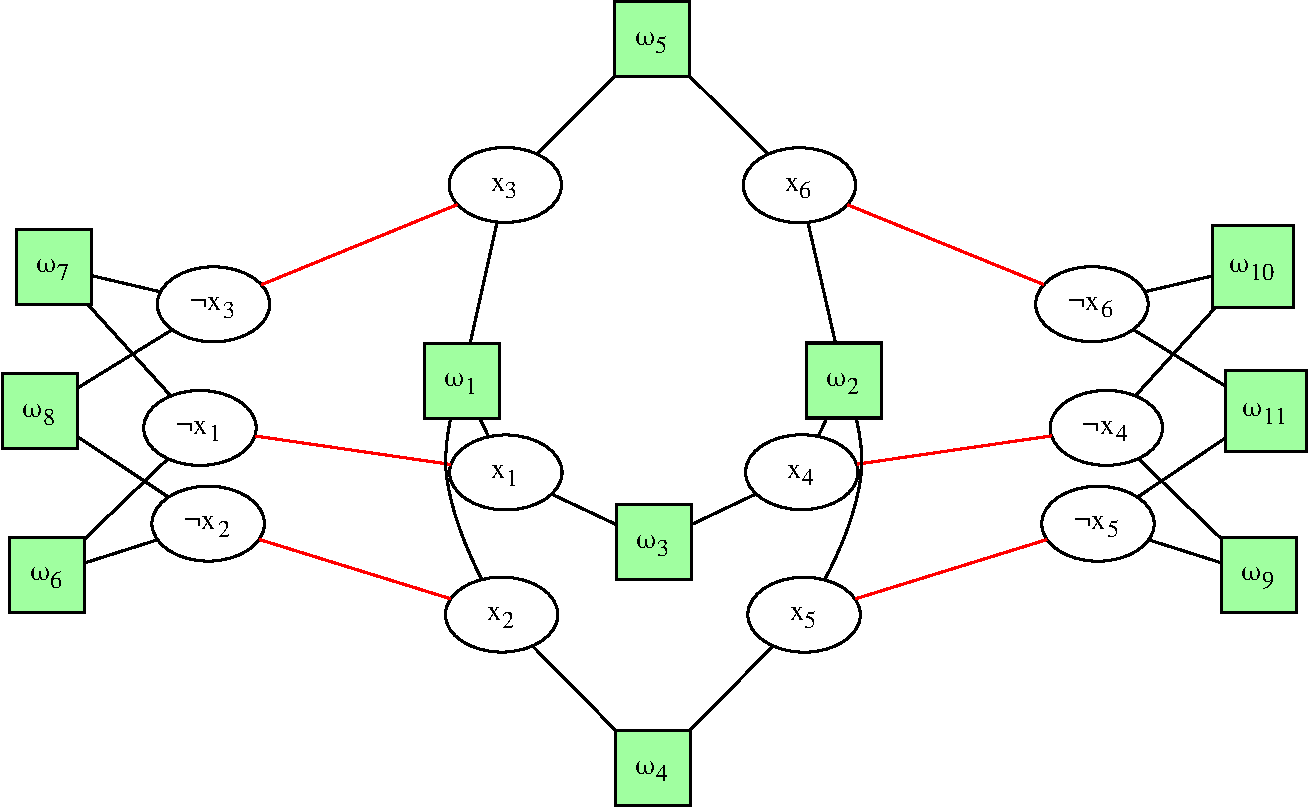
\includegraphics[width=4.3in]{cnfs/graph_cnf_no_opt-crop}
	\end{minipage}
 \caption{Example of constructed symmetry graph for a given CNF}
 \label{fig:graph_no_opt}
\end{figure}


\Cref{fig:graph_no_opt} shows the graph representation of a CNF. This problem have 12 variables and 21
clauses. So, the graph will have  24  + 21 = 45 vertexes where 24 represents literals vertexes (circle in the figure ) 
and 21 represents number of clause vertexes (square in the figure). The graph will also have 24 edges for boolean 
consistency (\hakan{XXX} color in the figure) and 36 edges that relies clauses vertexes to the literals.


% and  24 + 36 = 60 
%
%\hakan{Explication du graph + informations num nodes num edges. Probleme reel battleship
%}
%
%The battleship problems place one  ship of size *** and two ships of size* in grid 3x4 \\
%1  2  3\\
%4  5  6\\
%7  8  9\\
%10 11 12\\
%
%one ship per row.\\
%
%Produced graph contains and = 60 edges 


An optimization of this graph is possible with the usage of binary clauses i.e. a clause with only two literals.
The clause node can be omitted and we connect the two literals. As we cannot distinguish between the optimized edge 
and boolean consistency edges, we must check if the produced permutations are spurious. 
To do so, as we ensure the permutation commutes with the negation it suffice to check:
$\forall x \in \support(g), g.\neg x = \neg g.x$.
Roughly speaking, we check if the image of the negation of $x$ is equals to the negation of the image of $x$, for each element $x$ in the support of the permutation.
This optimization allows to compute symmetries of the problem more efficiently.
In the previous example, the graph has deleted 12 nodes and 12 edges. More generally,
the graph removes as many nodes and edges as binary clauses on the formula.
\Cref{fig:graph_opt} represents the optimized version the graph.

\begin{figure}[h]
	\begin{minipage}[c]{.2\textwidth}
		\lstinputlisting[numbers=none]{cnfs/battleship-3-4-unsat.cnf}
	\end{minipage}
	\begin{minipage}[l]{.75\textwidth}
		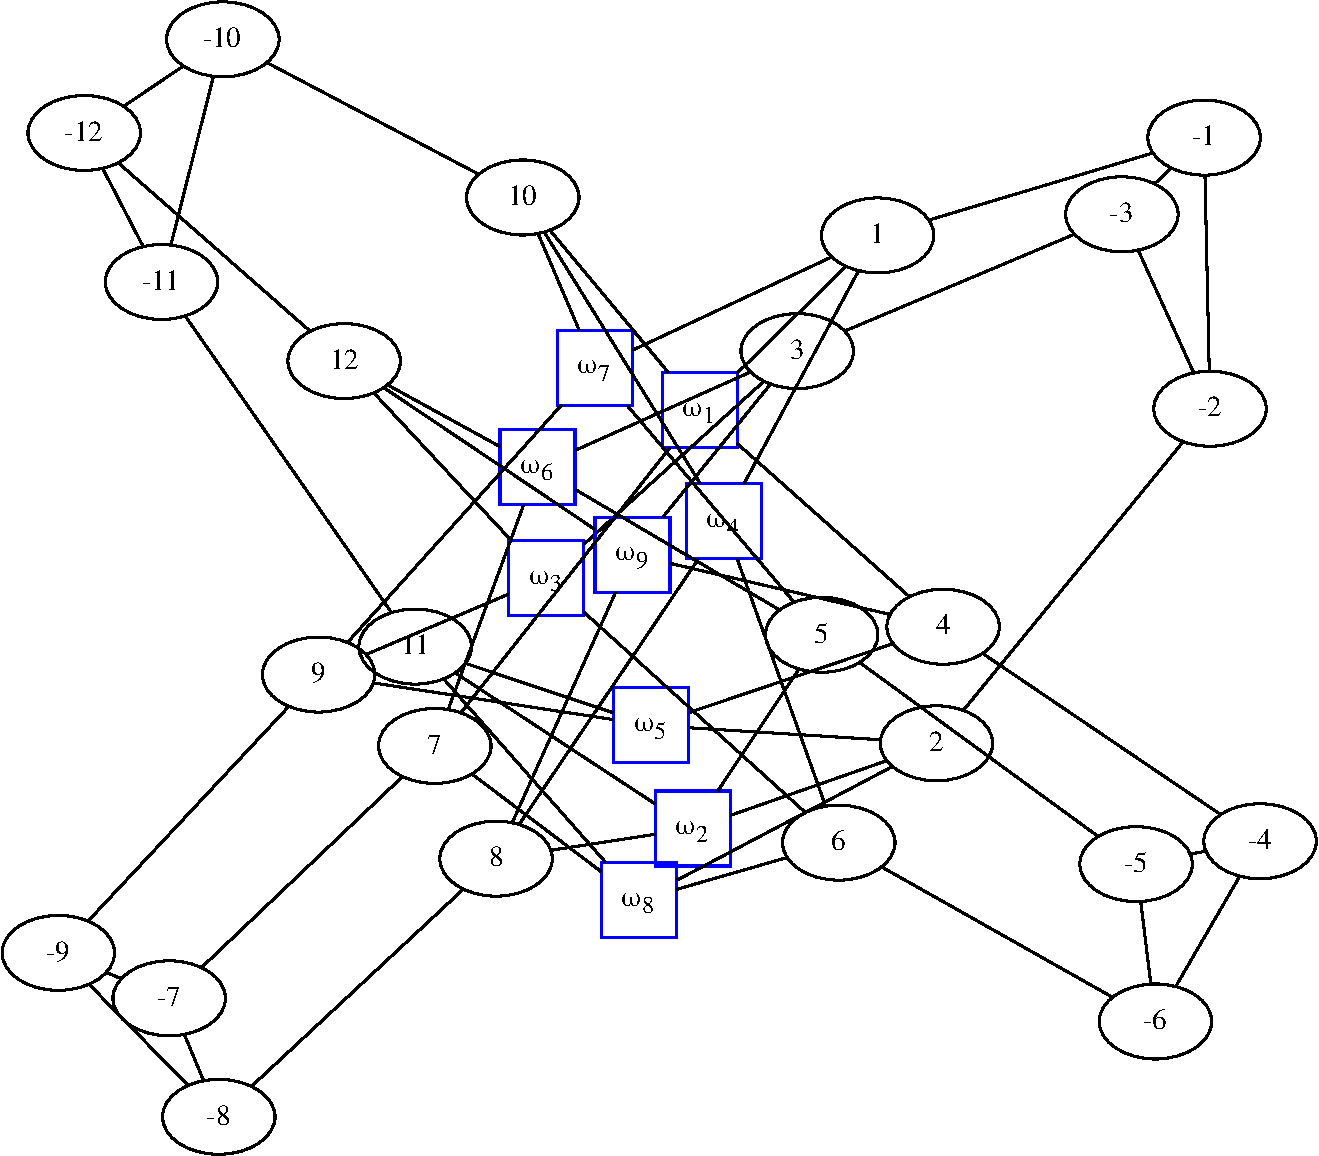
\includegraphics[width=4.3in]{cnfs/graph_cnf_opt-crop}
	\end{minipage}
	\caption{Example of constructed symmetry graph for a given CNF}
	 \label{fig:graph_opt}
\end{figure}


%\hakan{optimisation du graph}\\
%\hakan{creation d'un probleme fil conducteur and utilisation de celui dans chaque partie, du calcul des symétries
%jusqu'au SBP}\\

After the construction of a such graph, a graph automorphism tools take it as input and gives the set of generators as output.
With the previous graph, the following generators are obtained:

\begin{figure}
\begin{itemize}
	\item $g_1$: (2 3)(5 6)(8 9)(11 12)(-2 -3)(-5 -6)(-8 -9)(-11 -12)
	\item $g_2$: (4 5 6)(7 9 8)(-4 -5 -6)(-7 -9 -8)
	\item $g_3$: (4 7)(5 8)(6 9)(-4 -7)(-5 -8)(-6 -9)
	\item $g_4$: (1 2)(5 6)(7 9)(10 11)(-1 -2)(-5 -6)(-7 -9)(-10 -11)
	\item $g_5$: (1 10)(2 11)(3 12)(-1 -10)(-2 -11)(-3 -12)
\end{itemize}
\end{figure}




%The visualization of the orbits of literals on the problem could be seen in figure~\ref{fig:orbits}, where each node represents a literal. Two literals are 
%linked with an arc if it exists a permutation that maps the literal to the second one.
%By definition of the orbits, each literal belongs to a strongly connected components (SCC).
%
% \begin{figure}[h]
% 	\centering
% 		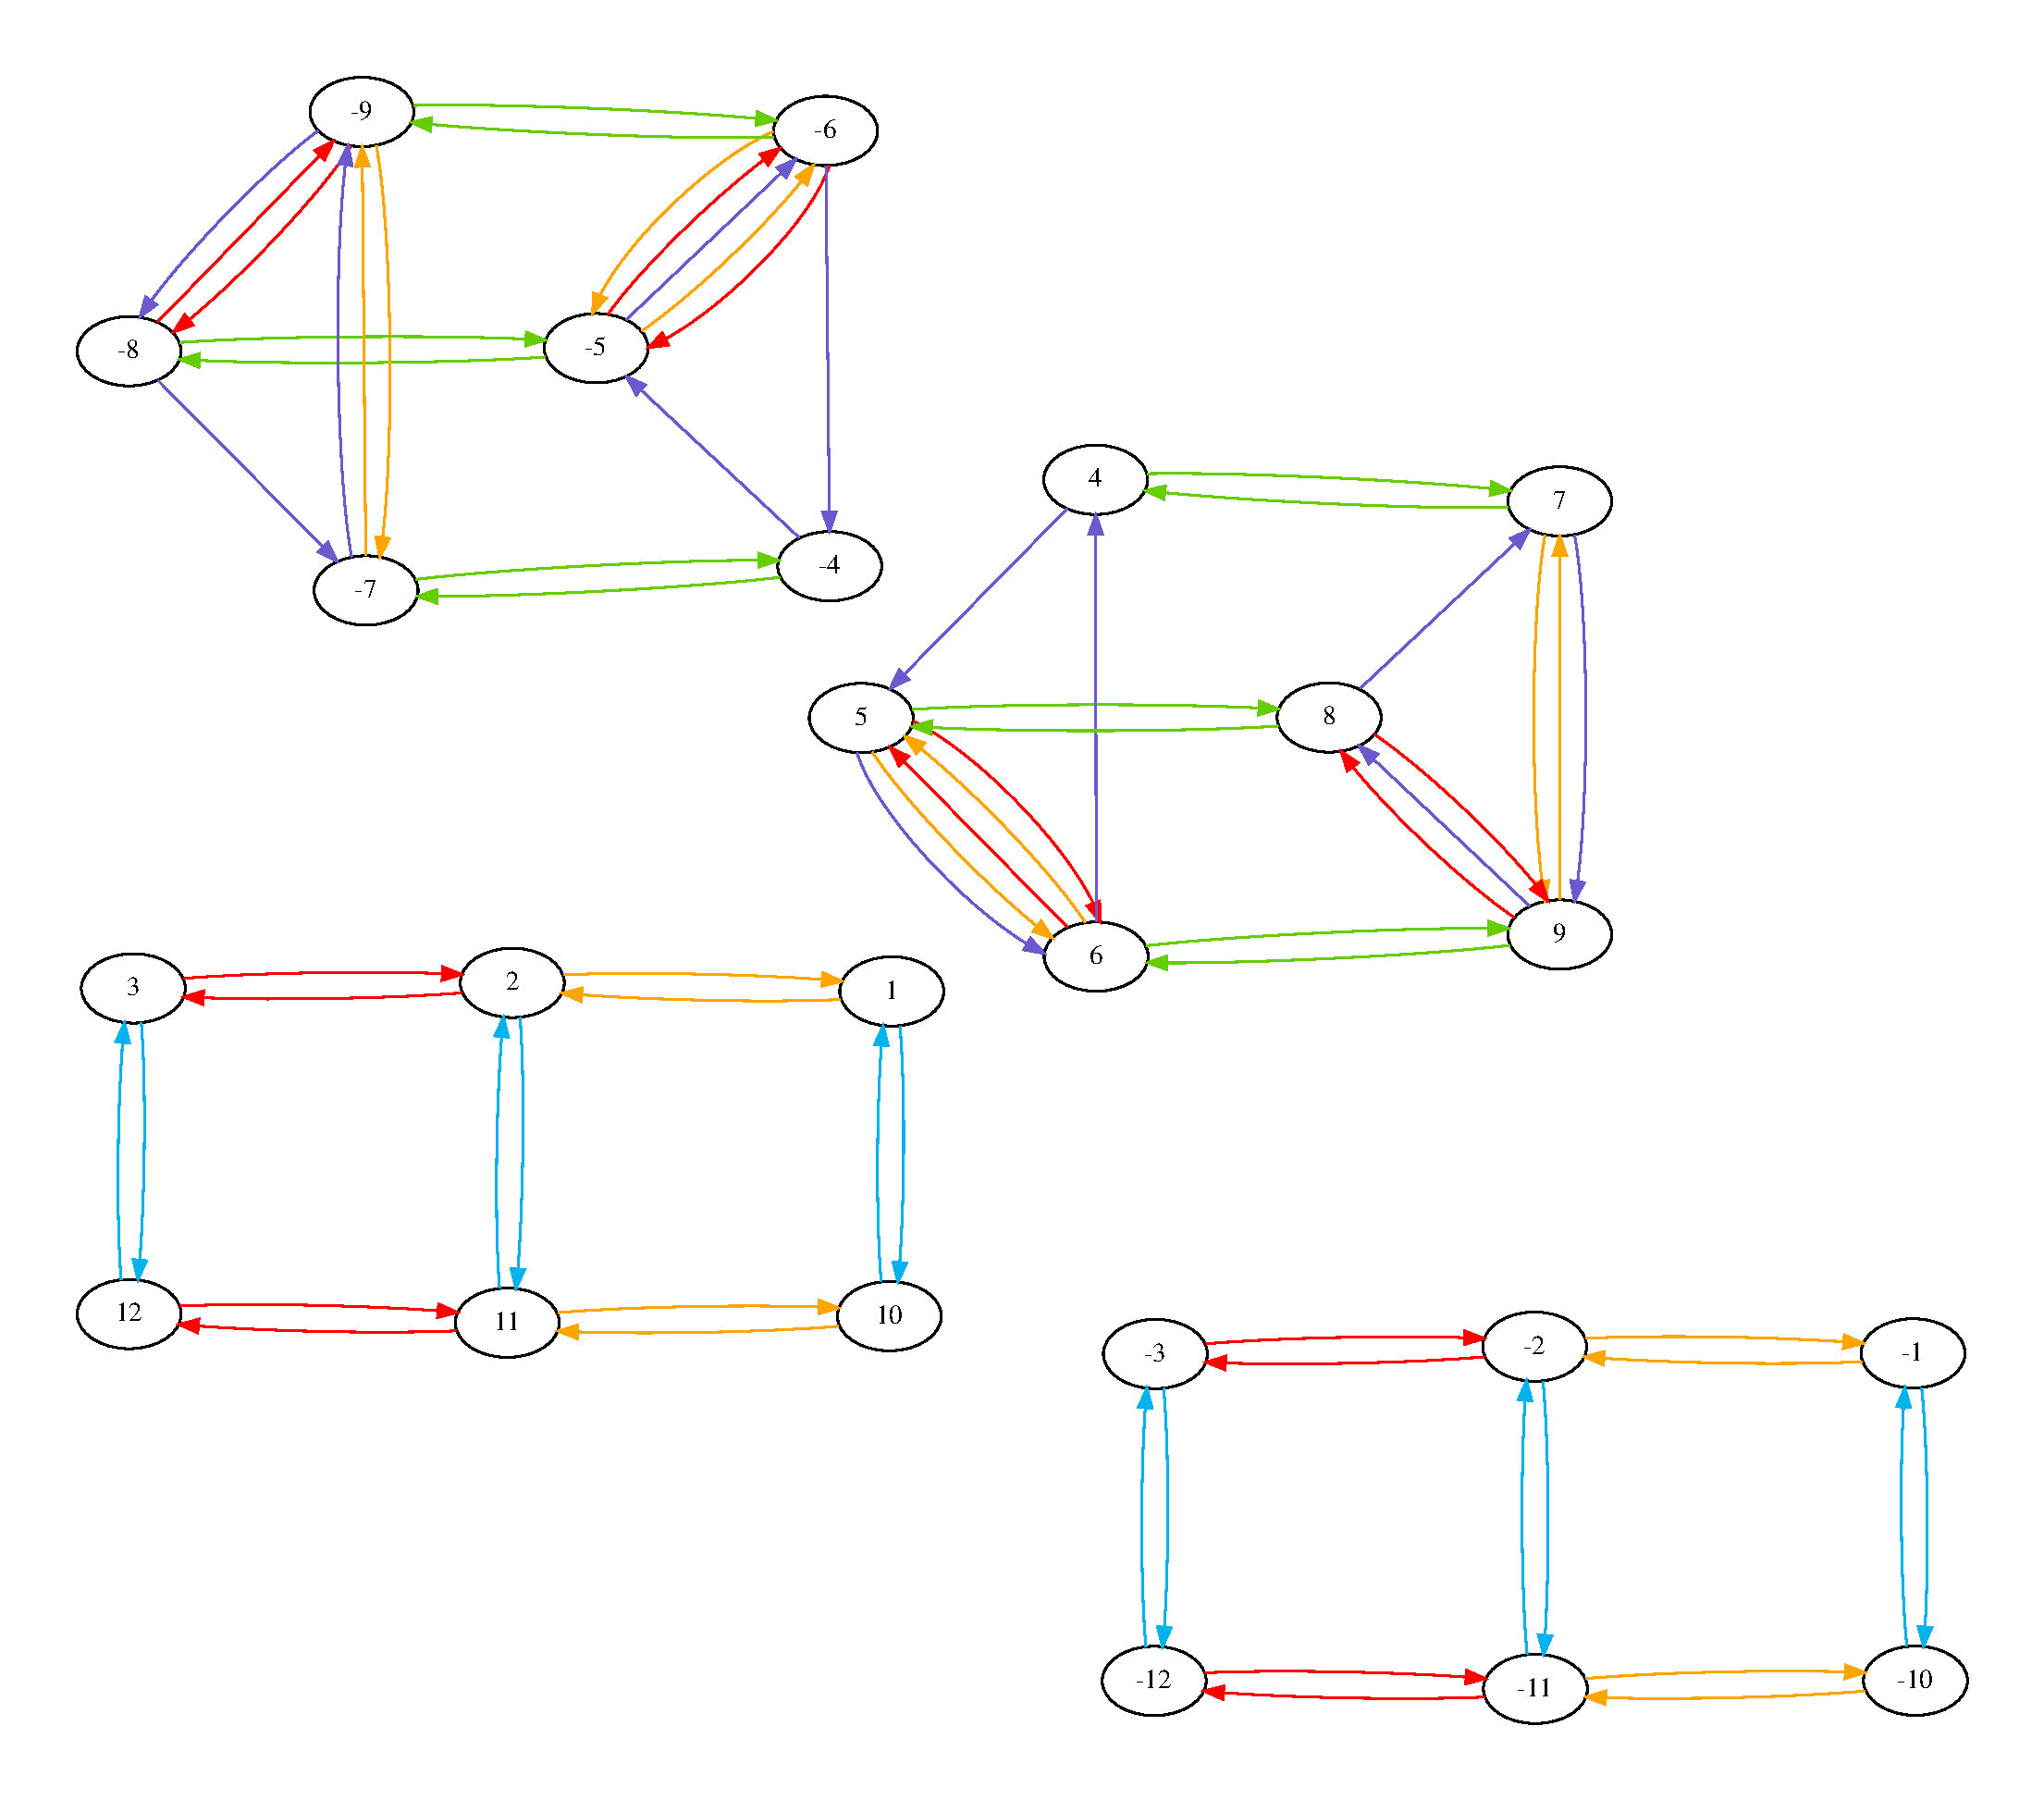
\includegraphics[width=\textwidth]{cnfs/orbits}
% 	\caption{Orbits}
% 	\label{fig:orbits}
% \end{figure}



\section{Usage of symmetries}

\emph{Symmetry breaking} aims at eliminating symmetry, either
by \emph{statically} posting symmetry breaking constraints that invalidate symmetric
assignments, or by altering the search space \emph{dynamically} to avoid symmetric search paths.


\subsection{Static symmetry breaking}

One way to exploit symmetry properties is to forbid equivalent assignment.
Let introduce an ordering relation between the assignments.

\begin{definition}[Assignments ordering]
	\label{def:assignment_ordering}
	We assume a total order, $\prec$, on $\Vars$.  Given two assignments $(\alpha,\beta) \in \Assignments(\Vars)^2 $, 
	we say that $\alpha$ is strictly smaller than $\beta$, noted $\alpha < \beta$, if there exists a variable $v \in \Vars$
	such that:
	\begin{itemize}
		\item for all $v' \prec v$, either $v' \in \alpha \cap \beta$ or $\neg v' \in \alpha \cap
		\beta$.
		\item $\neg v \in \alpha$ and $v \in \beta$.\footnote{We could have chosen as well $v \in \alpha$ and $\neg v \in \beta$ without loss of generality.}
	\end{itemize}
\end{definition}

Note that $<$ coincides with the lexicographical order on \emph{complete}
assignments. Furthermore, the $<$ relation is monotonic as expressed in the following proposition:

\begin{proposition}[Monotonicity of assignments ordering]
	\label{prop:monocity_assignments_ordering}
	Let  $(\alpha,\alpha',\beta,\beta') \in \Assignments(\Vars)^4 $ be four assignments.
	$$\text{If}~\alpha \subseteq \alpha'~\text{and}~\beta \subseteq \beta',~\text{then}~\alpha < \beta \implies \alpha' < \beta'$$
\end{proposition}

\begin{proof}
	The proposition follows on directly from Definition \ref{def:assignment_ordering}.
\end{proof}


Given a formula $\varphi$ and its group of symmetry $G$,
the \emph{orbit of $\alpha$ under $G$} (or
simply the \emph{orbit of $\alpha$} when $G$ is clear from the context) is the set
$ [\alpha]_G=\{ g.\alpha \mid g \in G \}$. 
The lexicographic leader (\textit{lex-leader} for short) of an orbit $[\alpha]_G$ is defined by
$min_<([\alpha]_G)$. This \textit{lex-leader} is unique because the lexicographic
order is a total order.
The optimal approach to solve a symmetric SAT problem would be to explore
only one assignment per orbit (for instance each lex-leader).To avoid exploring 
symmetry search space, \emph{symmetry breaking predicates}(SBP) are added to the formula.
These constraints are true only for the \emph{lex-leader} \cite{crawford1996symmetry}.
\Cref{fig:lex-leader} show different orbits and the lex-leader one.

\begin{figure}[!htbp]
	\centering
	%	\includegraphics[width=2in]{fig/assignment-lex-leader}
	\begin{tikzpicture}
    \tikzstyle{point}=[circle,draw,thick,fill=black,scale=0.2]
	\tikzstyle{point+}=[circle,draw=red,thick,scale=0.4]


\begin{scope}
\node[ellipse, draw, minimum width=4cm, minimum height=2cm] (c1) at (2.5,0){};
	\clip (2.5, 0) ellipse (2 and 1);
	\node[point+] (p2) at (1, 0.3){};
	\pgfmathsetseed{281}
	\foreach \p in {1,...,100}
	{
		\fill (4*rand,2*rand+0.25) circle (0.08);
	}
\end{scope}


\begin{scope}
\node[ellipse, draw, minimum width=4cm, minimum height=2cm] (c1) at (8.5,0){};
\clip (8.5,0) ellipse (2 and 1);
\node[point+] (p2) at (8.6, -0.1){};
\pgfmathsetseed{499478626}
\foreach \p in {1,...,40}
{
	\fill (4*rand+6,2*rand) circle (0.08);
}
\end{scope}

% Legend

\path[draw] (-1, -1.5) -- (13, -1.5);
\node[draw,ellipse, draw, minimum width=4cm, minimum height=2cm, scale=0.1] (ld) at (0, -2) {};
\node[align=left, text width=2.2cm] at (1.5, -2) {Orbit};


\node[circle, fill=black, draw=black, line width=0.5mm, scale=0.3] (lz) at (3, -2) {};
\node[align=left, text width=2.2cm] at (4.5, -2) {Assignment};


\node[point+] (le) at (7, -2) {};
\node[align=left, text width=4.2cm] at (9.5, -2) {Lex-leader assignment};

\path[draw] (-1, -2.7) -- (13, -2.7);



\end{tikzpicture}
	\caption{Show lex-leader per orbit}
	\label{fig:lex-leader}
\end{figure}




Generation of these lex-leaders constraints proposed by Crawford et al.~\cite{crawford1996symmetry}:

$$\forall i : (\forall j < i : x_j \Leftrightarrow g.x_j) \Rightarrow \neg x_i \vee g.x_i$$

Roughly speaking, assuming the ordering in \Cref{def:assignment_ordering}, for one permutation, these constraint express that 
the value of the variable $x_i$ must be smaller or equal than the value of $g.x_i$ and all variables $x_j$ that respect the constraint
$x_j \prec x_i$,  must have the same value of its symmetric. As such, these constraints encodes a valid lex leader with respect to 
this permutation. 



\begin{figure}

total order $ x_1 \prec x_2 \prec x_3 \prec x_4 \prec x_5 \prec x_6$\\
permutation $g_1 = (x_2 \enskip x_3)(x_5 \enskip x_6)(\neg x_2 \enskip \neg x_3)(\neg x_5 \enskip \neg x_6)$\\


$x_2 \preceq x_3$ \\
$x_2 = x_3 \implies x_5 \preceq x_6$\\

%2 == 3 -> 3 <= 2
%2 == 3 \land 3 == 2 -> 5 <= 6
\end{figure}







\begin{theorem}[Satisfiability preservation SBPs]
	\label{theorem:satisfiability_preservation_SBPs}
	Let $\varphi$ be a formula and $\psi$ the computed \textit{SBPs} for the set of
	symmetries $S(\varphi)$
	
	$$\varphi~and ~\varphi \wedge \psi \text{ are equi-satisfiable}.$$
\end{theorem}

\begin{proof}
	If $\varphi \wedge \psi$ is SAT then $\varphi$ is trivially SAT. If
	$\varphi$ is SAT, then there is some assignment $\beta$ that satisfies $\varphi$.
	Without loss of generality, $\beta$ can be chosen to be the lex-leader of its
	orbit under $S(\varphi)$. Thus, $g$ does not contradict $\beta$, which implies that
	$\beta \models \psi$.
\end{proof}

 


However, finding the lex-leader of an orbit is computationally hard~\cite{Luks2004}.
It exists two kind of symmetry breaking, the first one is \emph{full symmetry breaking} and it 
aims to visit exactly one assignment per orbit (generally the lex-leader). This
approach is in practice infeasible in the most case due to the exponential number of permutations in a group.
The second one is \emph{partial symmetry breaking} and it aims to visit at least one assignment per orbit. This approach is easy to set up and bring us to considerable reduction of the search spaces. The used set
of permutations is generally the set of generators of a formula given by the automorphism tool.


\hakan{Faire une section pour ça}
An extremely important point is the chosen lexicographic order.
Variable ordering may impact the number of generated constraint and so the performance of
the underlying SAT solver. Different orders are studied in the literature. 
One of the simplest order was the sorted variables according to their numbers.
Some others orders exists and exploit structural properties of the 
problem. In particular, the orbits of the variables in different ways. For example, the variables are chosen 
with their number of occurrences in the initial problem. This order, is equivalent to put largest orbit first
and so on, because each variable on the same orbit must have the same number of occurrences.
Another example of exploiting structural property of the orbit is the usage of \emph{stabilizer}.
The order choose a variable which maximize the number of stabilized permutations, removes the not stabilized ones and loop over until the empty set. The remaining variables are added to the order to get a complete order.



The exploitation of symmetries statically is called \emph{static symmetry breaking}.
It acts like a preprocessor which add \emph{symmetry breaking predicates} (SBPs) at the 
original formula and solve the augmented problem. 
This approach gives good performances in practice.

\hakan{Generation des clauses de SBPs}\\
\hakan{Parler des groupes speciaux  (totaux) }\\
\hakan{Generation des clause binaires breakid lie aux orbits}\\
\hakan{Parler de BreakID all in one tout au dessus}\\

\hakan{Put a complete exemple}\\

\hakan{Mettre des courbes}\\
\hakan{Tableau sur le nombre de sbp genere}\\

\hakan{ Shatter, BreakID}

\hakan{Conclu static}

In the general case,
the size of the \textit{sbp} can be exponential in the number of variables of
the problem so that they cannot be totally computed. The underlying SAT solver can 
 Even in more favorable
situations, the size of the generated \textit{sbp} is often too large to be
effectively handled by a SAT solver~\cite{Luks2004}. On the other hand, if
only a subset of the symmetries is considered then the resulting search pruning
will not be that interesting and its effectiveness depends heavily on the
heuristically chosen symmetries \cite{biere2009handbook}.



\hakan{Drawbacks de la methode pourquoi on fait du dynamique}

\subsection{Dynamic symmetry breaking}


Another disadvantage is that the solver is influenced by SBPs and explore the search space with a different 
manner and can affect performance negatively \hakan{FIND A REF}

In the literature, different approach of dynamic symmetry breaking are used to reduce the search space
of the sat solver in different ways. Some of them \textit{inject} constraints to allow only one representative assignment of each orbit like the static approach and others accelerate the propagation of variable using symmetrical properties. In this section, we present different approach to use symmetrical properties of a problem 
dynamically.


\subsubsection{SymChaff}

One of the first dynamic symmetry breaking approach is \emph{SymChaff}~\cite{sabharwal2005symchaff}
and is applicable only on special groups where all couple of variables are symmetric.
The idea of this approach is to treat each orbit like a \emph{symbolic variable}, i.e. instead of considering a single
variable, all symmetric variables are considered at the same time and so backtracked at the same time.
In this special case of groups the number of orbits is easy to compute but the order in which they would be
applied has a tremendously impact of the solver performance.
In the general case, when we take any groups computing the number of orbit will be very difficult and this approach
will be intractable.


\subsubsection{Symmetry Propagation}

A different approach can be used to reduce search space using symmetries is \emph{symmetry propagation}~\cite{Devriendt12}.
The general idea of this approach is to propagate symmetrical literals of those already propagated.
In other words, it accelerate the tree traversal by ``transforming some guessing (decisions) to deductions (propagation)''.
Indeed, problem that presents symmetries makes possible to deduce some value 
for the variables that would be guessed if symmetry properties were ignored.
These deductions will reduce the overall tree traversal depth and hence eventually accelerate the solving process.

To explain this approach, some definitions are required.

\hakan{Mettre logical conqequence quand on explique CDCL + Expliquer CDCL plus en detail avec les learnt et les raisons}

\begin{definition}[Logical consequence]
	\label{def:logical_consequence}
	A formula $\phi$ is a logical consequence of a formula $\varphi$ denoted by $\varphi \models \phi$ if for all assignment
	$\alpha$ satisfying $\varphi$, it satisfies also $\phi$. Two formulas are \emph{logically equivalent} if each is a logical
	consequence of the other.
\end{definition}

\begin{proposition}[Symmetry propagation]
	\label{prop:symmetry_propagation}
	Let $\varphi$ be a formula, $\alpha$ an assignment and $l$ a literal. 
	If $g$ is a symmetry (permutation) of $\varphi \cup \alpha$ and
	$\varphi \models \{l\}$, then $\varphi \cup \alpha \models g.\{l\}$ is also true.
\end{proposition}

In other words, if a literal $l$ was propagated by the solver and $g$ is a \emph{valid} symmetry for the
sub problem $\varphi \cup \alpha$ (in which all satisfied clauses and false literals are removed), so , the solver can
also propagate the symmetrical of $l$. The problem here is to determinate which symmetries are valid for the formula
$\varphi \cup \alpha$.

\begin{definition}[Active symmetry]
	\label{def:active_symmetry}
	A symmetry $g$ is called active under a partial assignment $\alpha$ $\text{if } g.\alpha = \alpha$
\end{definition}

The Definition~\ref{def:active_symmetry} leads to the following proposition:

\begin{proposition}
	\label{prop:active_symmetry}
	Let $\varphi$ a formula and $\alpha$ a partial assignment. Let $g$ a symmetry of $\varphi$,
	if $g$ is active under the assignment $\alpha$, then $g$ is also a symmetry of $\varphi \cup \alpha$
\end{proposition}

The previous proposition states that an active symmetry $g$ for a partial assignment $\alpha$ still valid for
the formula $\varphi \cup \alpha$. So when a literal $l$ is propagated, and a symmetry $g$ is active for a
partial assignment $\alpha$, the solver can also propagate $g.l$. 
Moreover, the group theory allow to compose permutations with the composition operator~$\circ$ and the composition of two active symmetries is also an active symmetries so the solver can also propagate $g^2.l, g^3.l, ... $

\hakan{Peut etre expliquer les sym conflicts}

The authors of symmetry propagation improve the active symmetries, introducing \emph{weakly active} symmetries.

\begin{definition}[Weakly active symmetry]
	\label{def:weakly_active_symmetry}
	Let $\varphi$ a formula and ($\delta, \alpha, \gamma$) a state of a CDCL solver in which $\delta$ is the set of decisions,
	$\alpha$ is the current assignment and $\gamma$ the reasons of the learned clauses. Then a symmetry $g$ is weakly active 
	if $g.\delta \subseteq \alpha$
\end{definition}

This definition leads to the following proposition:

\begin{proposition}
	Let $\varphi$ be a formula, $\alpha $ an assignment. If
	there exists a subset $\delta \subseteq \alpha $ and a symmetry $g$ of $\varphi$ such that 
	$g.\delta \subseteq \alpha $ and $\varphi \cup \delta \models \varphi \cup \alpha$, then $g$ 
	is also a symmetry of $\varphi \cup \alpha $.
\end{proposition}

\hakan{Proof}

In other words, we can detect with a minimal effort, the symmetries of $\varphi
\cup \alpha$ by keeping track of the set of variables $\delta$, which are 
in a state-of-the-art complete SAT solving algorithms, the set of decision variables.
Obviously, a weakly active symmetry can also propagate the symmetrical literals of a propagated one.
Moreover, weakly active symmetries allows more propagation and so is more efficient.
Note that if a weakly active symmetry want to propagate a symmetrical literal which are already affected to the 
opposite value, this leads to a symmetry conflict and the solver backtracks to propagate the symmetrical value correctly.

\hakan{Mettre des tableaux, courbes etc ...}
\hakan{Courbe VS static an no sbp}\\
\hakan{Conclu SP, depend on the solver choice}

Symmetry propagation gives good performances on many symmetric instances.
The overall performance of the symmetry propagation is intrinsically related to the decision heuristics of
the underlying SAT solv1er.

One optimization of symmetry propagation is the following proposition, as seen in Section
\hakan{DETERMINE SECTION SAT LEARNING} each propagated clause has a reason which is an assertive clause.
If the symmetrical clause is also an assertive one, this clause can be added in the formula without any requirements
(even if the permutation is not weakly active). The added symmetrical clause will participate also to unit propagation and propagate the symmetrical literal.


\subsubsection{Symmetry Explanation Learning}


Another approach to exploit symmetry without removing any satisfiable assignment of the problem
is \emph{Symmetry Explanation Learning}~\cite{devriendt2017symmetric}. This approach aim to learn useful 
symmetrical variant of clauses only where they are used by the solver. A useful clause is a clause that participate
to the unit propagation or conflict. 
A naive approach to ensure that is to compute the symmetrical clause of 
each learned clauses and check if it is useful. In addition, due to size of a group a clause can have many 
symmetrical ones. the naive approach will have an important overhead and will be intractable on reel problems.
SEL have different optimization based on the following facts. First,
On the unit propagation, propagated literals has a reason clause which are assertive, and in the general case,
 symmetries permutes only few literals of the clause so symmetrical clauses can also be assertive and so useful.
Secondly, avoiding to add identical clauses to the problem, symmetrical clauses ares stored in different learning scheme and used when classical unit propagation is finished. This ensure that no duplicate clause is added in the problem.
  

 





%\begin{proposition}[Satisfiability preservation]
%	\label{prop:equi_satisfiability}
%	 Let $\varphi$ a CNF problem and $\psi$ the computed symmetry breaking predicates.
%	 Solve $\varphi \cup \psi$ is equi-satisfiable to solve $\varphi$.
%\end{proposition}
%
%\begin{proof}
%	On the first case, if the initial formula $\varphi$ is \unsat,
%	then the augmented problem $\varphi \cup \psi$ is trivially \unsat.
%	On the second case, if $\varphi$ is \sat then $\varphi \cup \psi$ is also \sat because 
%	$\psi$ forbids only non lex-leader assignment so the formula still be \sat.
%\end{proof}



%% Local Variables:
%% TeX-master: "main.tex"
%% ispell-dictionary: "en_US"
%% mode: latex
%% mode: flyspell
%% coding: utf-8
%% End:
